\subsection{Author-workstation full-factorial search results}
\label{sec:windows-full-s-results}

The numerical investigations were extended using the author's complete
Windows-machine \texttt{full} run. The original archived experiment contains
$80\,640$ search records: $n\in\{24,48\}$, difference orders
$d=0,\ldots,5$, the two fixed means $\mu=0$ and $\mu=0.15$,
five selection criteria (CV, GCV, AICc, BIC, conditional marginal MLE),
seven numerical solver implementations, and $R\in\{1,3,8\}$
independent observed series, with cold and shared backend preparation.
The eight computational policies distinguish one evaluation, three
complete 17-point finite-grid searches, and two bounded
\emph{local} continuous searches. Two seeds were executed and every
configuration was timed with seven repetitions and one BLAS thread.
This is a separate physical machine and experimental design from
the earlier hosted-Linux reference figures.

The normalized-smoothness grid includes the exact $S=0$ and $S=1$
endpoints together with an increasingly fine near-one tail through
$S=0.999999999999$. The exact $S=1$ endpoint corresponds to
$\lambda=\infty$ and is scored analytically; it is not a request to
factor an infinite-penalty matrix. Numerical instability at extreme
finite penalties and statistical inapplicability are recorded
separately; MLE for $d=0$ is outside the adopted likelihood model.

Both the \emph{native $S$} grid and the \emph{premapped $S\to\lambda$}
grid sample the identical 17 candidate penalties, so they must
agree in criterion scores and selected smoothness. The independently
spaced log-penalty grid uses equal candidate count and outer finite
endpoints but \emph{different interior candidates}. Only the two
matched grids can support a pure computational-speed comparison
at a fixed discrete statistical estimator. For pretranslation we
charge the one-time inverse-grid construction exactly once to
a standalone search; repeated cross-criterion uses can amortize it.

% AUTO-GENERATED FROM TWO RECORDED WINDOWS SEEDS; DO NOT EDIT VALUES
\begin{table}[tbp]
\centering
\caption{Author's Windows full-run median complete 17-point grid
selection times (milliseconds) for two independent recorded seeds,
$n=48$, $d=2$, fixed $\mu=0$, $R=1$, spectral SVD,
one BLAS thread and seven timing repetitions.
Premapped $S\to\lambda$ includes one complete grid conversion.
Independent log-$\lambda$ has different interior nodes.
Cells are shown only where both seeds are numerically valid.}
\label{tab:windows-full-search}
\begin{tabular}{lrrr}
\toprule
Criterion & Native $S$ & Premapped $\lambda$ & Log-$\lambda$ \\
\midrule
CV & 2.004 & 1.879 & 0.545 \\
GCV & 1.851 & 1.800 & 0.426 \\
AICc & 1.887 & 1.810 & 0.458 \\
BIC & 2.016 & 1.810 & 0.449 \\
MLE & 3.477 & 2.035 & 0.515 \\
\bottomrule
\end{tabular}
\end{table}

When reusing exactly one pretranslated candidate grid across all five criteria, the measured native-$S$ total was 11.234\,ms and the shared $S\to\lambda$ mapping plus five backend-only searches took 3.980\,ms (descriptive ratio 2.823). This accounting charges grid inversion exactly once, not once per statistical criterion.

The $80\,640$ original author-host measurements and machine
metadata are preserved under
\texttt{paper/benchmarks/results/full\_s\_search\_modes/}.
The Windows study covers $n=24,48$, $d=0,\ldots,5$,
$\mu=0,0.15$, $R=1,3,8$, seven backends, five criteria,
and cold versus shared backend preparation.
MLE at $d=0$ remains not applicable. At $S=1$
the $\lambda=\infty$ limit is evaluated analytically.


\begin{figure}[tbp]
\centering
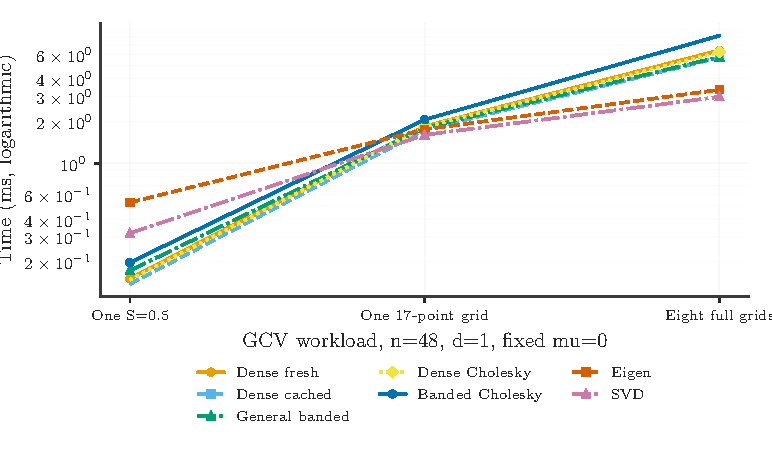
\includegraphics{figures/windows_full_s_workloads.pdf}
\caption{Full Windows-run comparison of one GCV evaluation at $S=0.5$,
one complete seventeen-point search and eight independent
complete searches ($n=48$, $d=1$, $\mu=0$). The vertical axis is
logarithmic and each backend is included only for workloads that
were numerically valid in both recorded seeds. Premapped standalone
times include the common grid inversion once.}
\label{fig:windows-full-workloads}
\end{figure}

\begin{figure}[tbp]
\centering
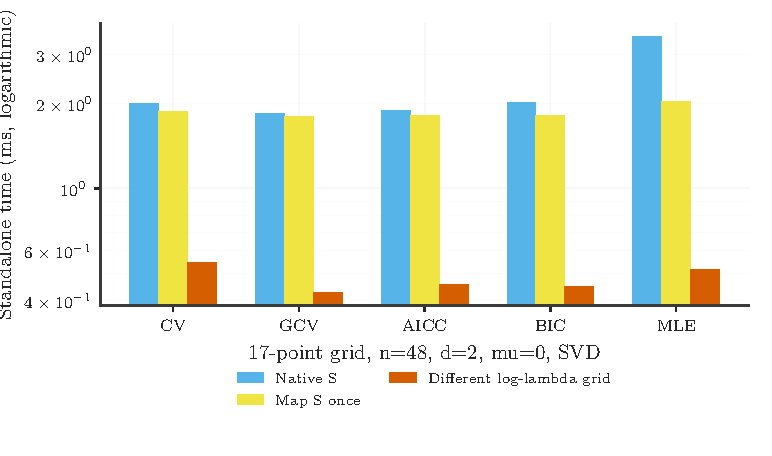
\includegraphics{figures/windows_full_s_grid_coordinates.pdf}
\caption{Observed Windows elapsed time for five existing selection
criteria under native $S$, a once-premapped $S$ grid evaluated in
$\lambda$, and an independently sampled log-$\lambda$ grid
($n=48$, $d=2$, $R=1$, $\mu=0$, spectral SVD). Premapping is charged
once to the standalone time. The third policy samples different
interior penalty candidates, so runtime alone does not establish
statistical superiority. The vertical axis is logarithmic.}
\label{fig:windows-full-grid}
\end{figure}

\begin{figure}[tbp]
\centering
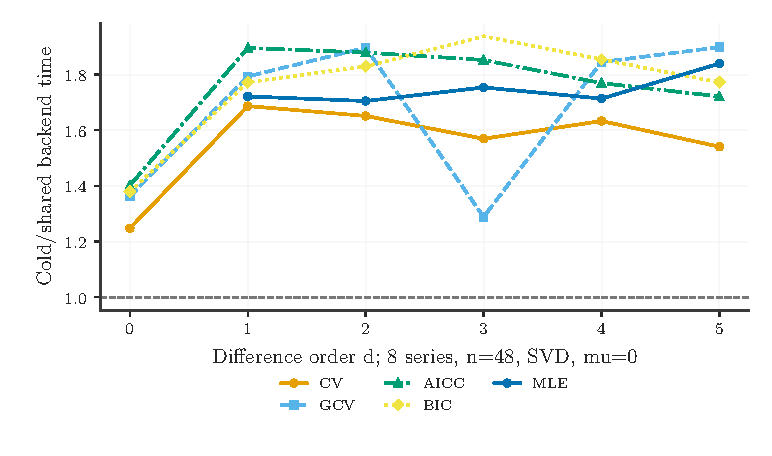
\includegraphics{figures/windows_full_s_reuse_d.pdf}
\caption{Cold-to-shared backend-only runtime ratio for repeated
$R=8$ full-grid searches across orders $d=0,\ldots,5$
($n=48$, fixed $\mu=0$, SVD). The ratio is shown only when
both experimental seeds satisfy each criterion's numerical
validity requirements. Shared spectral preprocessing can be
amortized across series, but does not make the grid itself
or matrix factorization cost free.}
\label{fig:windows-full-reuse}
\end{figure}

\begin{figure}[tbp]
\centering
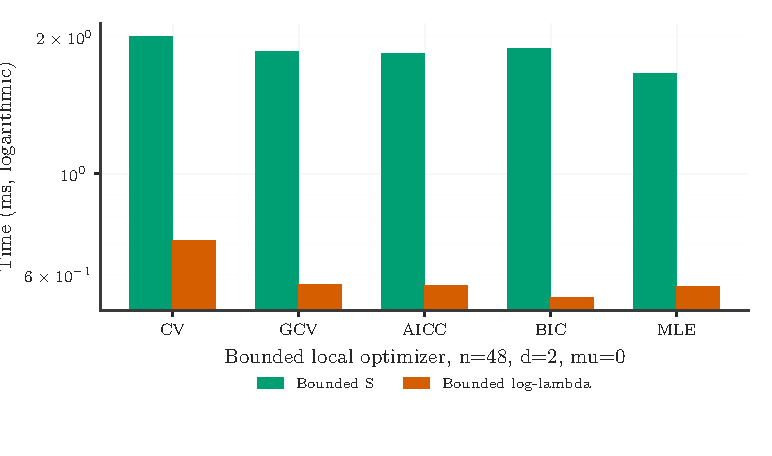
\includegraphics{figures/windows_full_s_bounded.pdf}
\caption{Measured bounded \emph{local} scalar optimization in the
smoothness coordinate $S$ and in $\log\lambda$
($n=48$, $d=2$, $\mu=0$, SVD), including analytical endpoint
checks. Function-evaluation counts and candidate positions
can differ; a bounded optimizer does not certify a global
criterion minimum. The ordinate is logarithmic.}
\label{fig:windows-full-bounded}
\end{figure}

\begin{figure}[tbp]
\centering
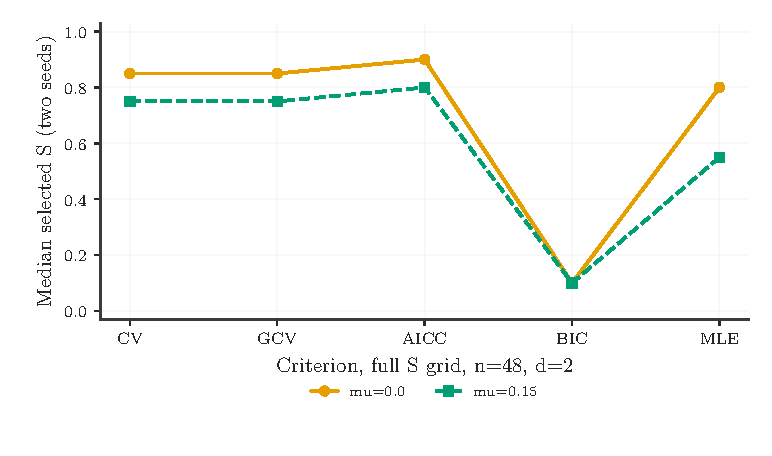
\includegraphics{figures/windows_full_s_means.pdf}
\caption{Median selected normalized smoothness for each statistical
selection criterion under the \emph{same mapped} seventeen-point
candidate grid, contrasting fixed $\mu=0$ and $\mu=0.15$
($n=48$, $d=2$, spectral SVD, two experimental seeds). Only
validated solutions appear; the criterion values themselves have
different scales and must not be compared across criteria.}
\label{fig:windows-full-mu}
\end{figure}

All timings are empirical medians under the recorded Windows machine
and software configuration; the source CSV, grid-construction records,
and environment metadata are retained unmodified. Automatically
derived two-seed aggregates, selected-parameter summaries, numerical
parity checks, the data-driven table above and all AwesomeFigures
PDF/SVG artwork are committed separately under
\texttt{paper/benchmarks/windows\_full\_s\_analysis/}.
They neither supersede the hosted-Linux reference measurements nor
demonstrate improved out-of-sample forecast accuracy, a new
smoothing criterion, or a universally optimal numerical backend.
